%%%%%%%%%%%%%%%%%%%%%%%%%%%%%%%%%%%%%%%%%%%%%%%%%%%%%%%%%%%%%%%%%%%%%%%%%%%%%%%%
%2345678901234567890123456789012345678901234567890123456789012345678901234567890
%        1         2         3         4         5         6         7         8

\documentclass[letterpaper, 10 pt, conference]{ieeeconf}  % Comment this line out if you need a4paper

%\documentclass[a4paper, 10pt, conference]{ieeeconf}      % Use this line for a4 paper

\IEEEoverridecommandlockouts                              % This command is only needed if 
                                                          % you want to use the \thanks command

\overrideIEEEmargins                                      % Needed to meet printer requirements.

%In case you encounter the following error:
%Error 1010 The PDF file may be corrupt (unable to open PDF file) OR
%Error 1000 An error occurred while parsing a contents stream. Unable to analyze the PDF file.
%This is a known problem with pdfLaTeX conversion filter. The file cannot be opened with acrobat reader
%Please use one of the alternatives below to circumvent this error by uncommenting one or the other
%\pdfobjcompresslevel=0
%\pdfminorversion=4

% See the \addtolength command later in the file to balance the column lengths
% on the last page of the document

% The following packages can be found on http:\\www.ctan.org
\usepackage{graphics} % for pdf, bitmapped graphics files
\usepackage{epsfig} % for postscript graphics files
\usepackage{mathptmx} % assumes new font selection scheme installed
\usepackage{times} % assumes new font selection scheme installed
\usepackage{amsmath} % assumes amsmath package installed
\usepackage{amssymb}  % assumes amsmath package installed
\usepackage{cite}

\title{\LARGE \bf
Toward Human-Robot-Teaming for Mobile Robot Navigation Using
 Remote control,  Digital Twin, and  Transversability Map
}


\author{Trung Kien La$^{1}$ and Eric Guiffo Kaigom$^{1}$% <-this % stops a space
%\thanks{*This work was not supported by any organization}% <-this % stops a space
\thanks{$^{1}$The authors are with the Deptartment of Computer Science \& Engineering,
        Frankfurt University of Applied Sciences, 60318 Frankfurt am Main, Germany, e-mails:
        {\tt\small trung.la@stud.fra-uas.de; kaigom@fb2.fra-uas.de}}%
% \thanks{$^{2}$Eric Guiffo Kaigom is with Deptartment of Computer Science \& Engineering,
% Frankfurt University of Applied Sciences, 60318 Frankfurt am Main, Germany
%         {\tt\small kaigom@fb2.fra-uas.de}}%
}


\begin{document}



\maketitle
\thispagestyle{empty}
\pagestyle{empty}


%%%%%%%%%%%%%%%%%%%%%%%%%%%%%%%%%%%%%%%%%%%%%%%%%%%%%%%%%%%%%%%%%%%%%%%%%%%%%%%%
\begin{abstract}

Collision prediction and avoidance is essential for the autonomous navigation of mobile robots. A transversability map is a way to achieve this objective. However, this approach might fail when the environment is subject to  dynamic motion of living or artificial entities. Included are pedestrians, animals, and other vehicles that the robot cannot handle. In this paper, we  embrace this challenge by achieving a flexible human-robot teaming that leverages a shared control of the robot. A human operator can remotely supervise and actively guide the robot as well as  share or leave full control to the robot that autonomously moves toward a desired goal. For this purpose, a situation-aware control signal balances the input of the autonomous robot and the cognitive input of the  remote human operator. The robot employs a  transversability map to autonomously evolve in unstructured environments. In critical situations, the human operator can  intervene and seamlessly operate the robot from everywhere by using any web-capable device.  Such a human-in-the-loop control is realized through a bidirectional wireless communication between the physical robot and its multi-modal digital twin.  The human-robot teaming enhances the likeliness of a successful navigation even without pre-defined goal and dynamics obstacles. The paper outlines the conceptual architecture and shares preliminary results of our approach.

\end{abstract}


%%%%%%%%%%%%%%%%%%%%%%%%%%%%%%%%%%%%%%%%%%%%%%%%%%%%%%%%%%%%%%%%%%%%%%%%%%%%%%%%
\section{INTRODUCTION}
The navigation of mobile robot in unstructured environments requires the detection, interpretation, and avoidance obstacles. Combining  RGB and depth images, semantic segmentation,  intrinsic and extrinsic  camera parameters to predict a bird?s-eye-view transversability map is an approach to cope with obstacle during navigation \cite{wayfast}. The underlying model obtained through self-supervised training is fed with sensed images. It returns an array of parameters that describe the linear and angular  

Geometric navigation approaches that are for example LiDAR based, are especially limited outdoors \cite{wayfast}.
Self-supervised autonomous navigation systems such as BADGR \cite{BADGR}, WayFAST \cite{wayfast} or the successor model WayFASTER \cite{wayfaster}, are therefore used to estimate the traversability with regard to bumps and navigable objects such as tall grass.
Even though these camera-image based neural networks excel in a static environment, they are constrained in a dynamic and busy environment where people, animals or other objects such as cars are moving.
Furthermore, not all parameters can be taken into account in these models. Parameters such as battery state of charge (SoC) or engine temperatures of the robot are equally important to ensure successful and safe navigation.
It is therefore common for robots to be additionally monitored and controlled by a human operator.
For these reasons, it is advantageous for a person with better situational awareness to take back control for a certain action or period of time. 
In this respect, shared autonomy describes a robotic system that independently adapts its autonomy level to the given environmental factors \cite{phri}. 
To support this physical robot-human interaction (pHRI), intuitive control and monitoring of critical data is required. 
We therefore provide the robot operator with a web-based interface that reflects the perception of the robot, visualizes its critical data and offers multiple control options. 
Security aspects such as login and persistent data storage via a database are also integrated. 
In addition, a concept for shared autonomy with the Husky UGV mobile robotic platform from Clearpath \cite{husky} and WayFASTER are presented. 

\section{Web Framework}

The web framework is based on flask and is used to control and monitor the Husky, which runs on ROS2 Humble and is platform-independent. 
Bidirectional communication between human and the robot is provided by the rosbridge\_suite package [source].   
Due to the web-based approach, all devices with a browser can access the app, provided they are in the same local network as the robot.
Fig. \ref{fig:userapp} shows the backend architecture, ROS packages and other relevant information which were leveraged for developing the framework.
\begin{figure}[b]
    \centerline{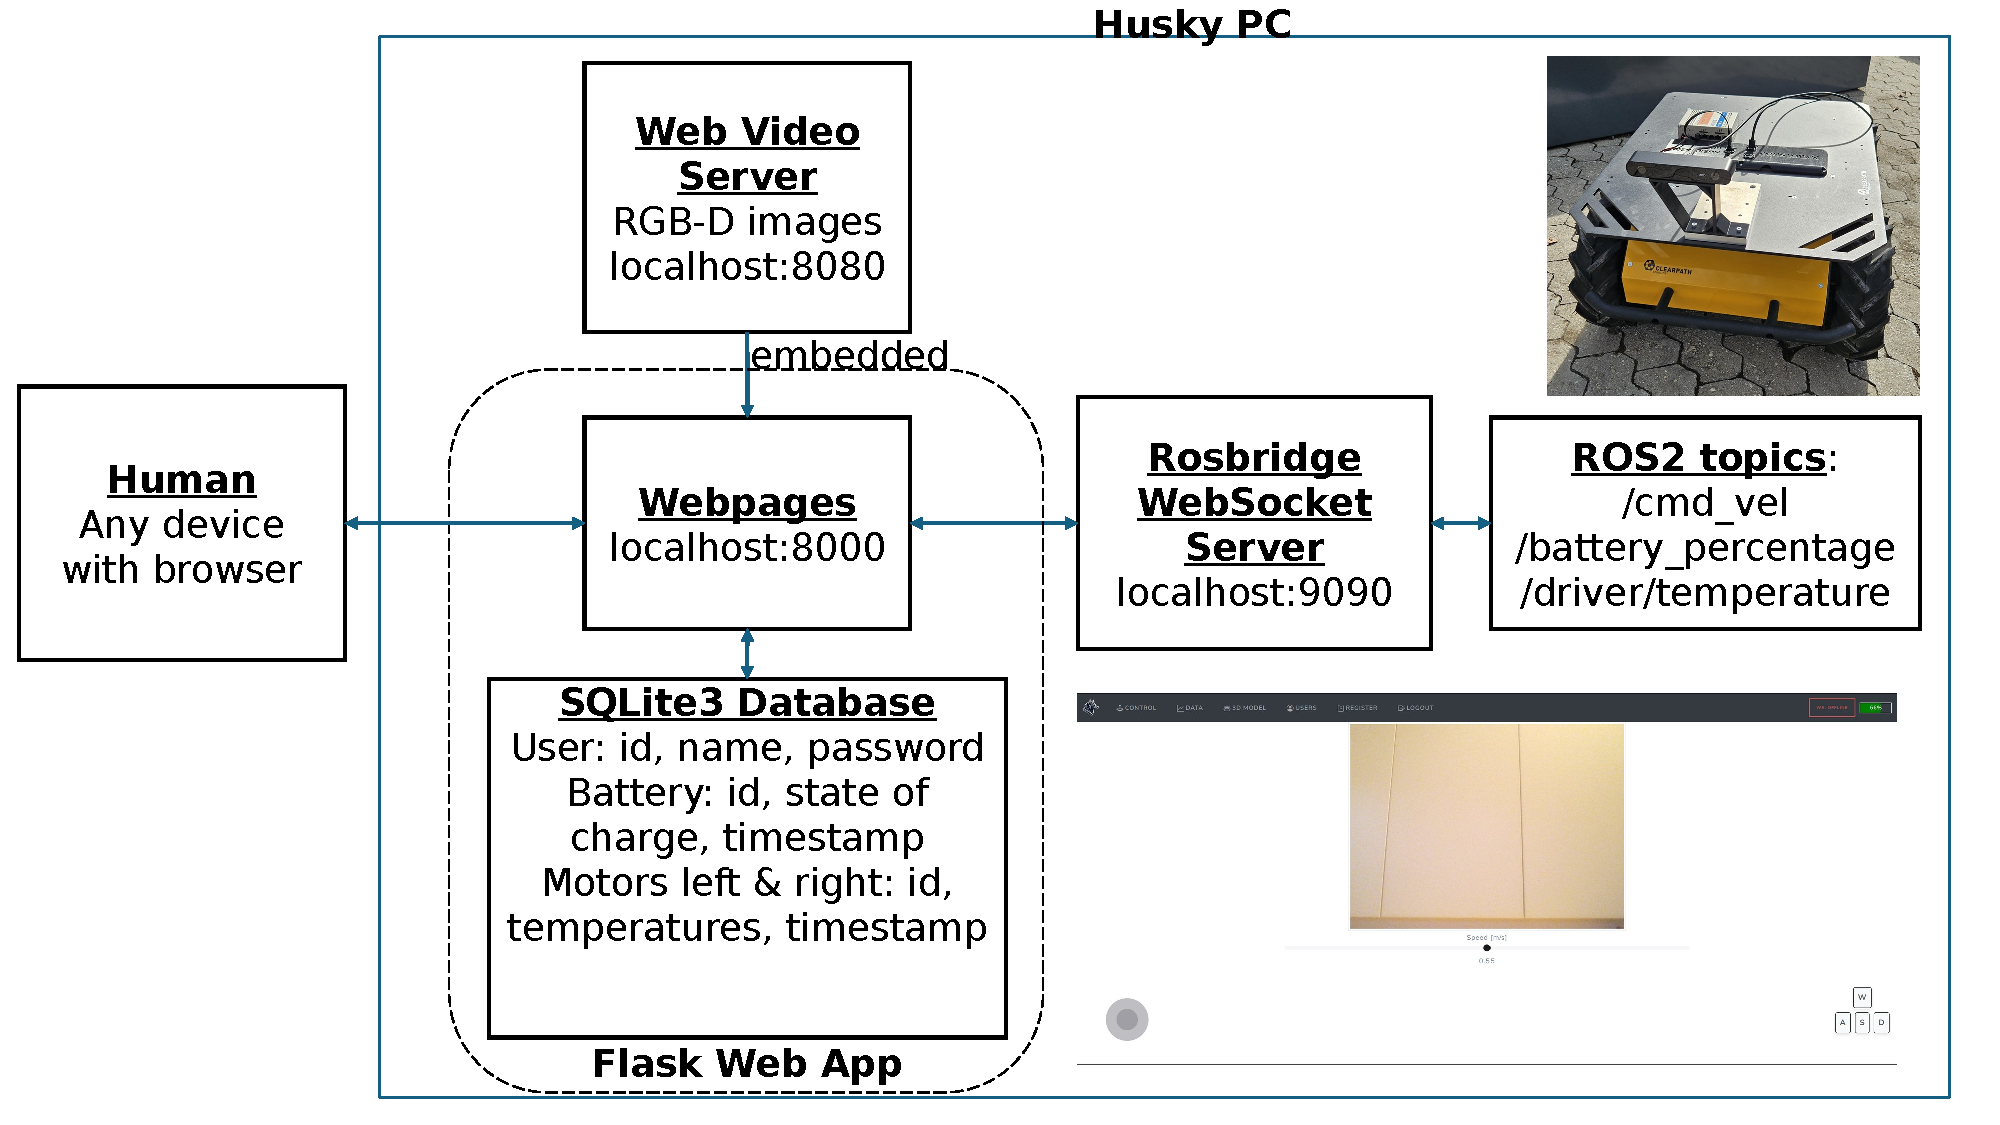
\includegraphics[width=8.9cm]{images/ROS_Web_App_Architecture.pdf}}
    \caption{Backend architecture of the web app and tools used.}
    \label{fig:userapp}
\end{figure}

\subsection{Control panel}
The control panel in Fig. \ref{fig:controlpanel} shows a live image stream (in the center) of a Zed2i camera attached on the Husky. Above the camera image, a navigation bar is located. 
Below the camera image there is a speed slider and two control elements such as a virtual joystick and virtual keyboard keys for controlling the Husky. 
In addition, the Husky can be controlled with a physical keyboard when the operator has access to the control panel. Keyboard control can be helpful in situations where precision is required compared to the joystick.
Other elements such as the battery SoC and the WebSocket connection are also shown embedded in the navigation bar.
\begin{figure}[t]
    \centerline{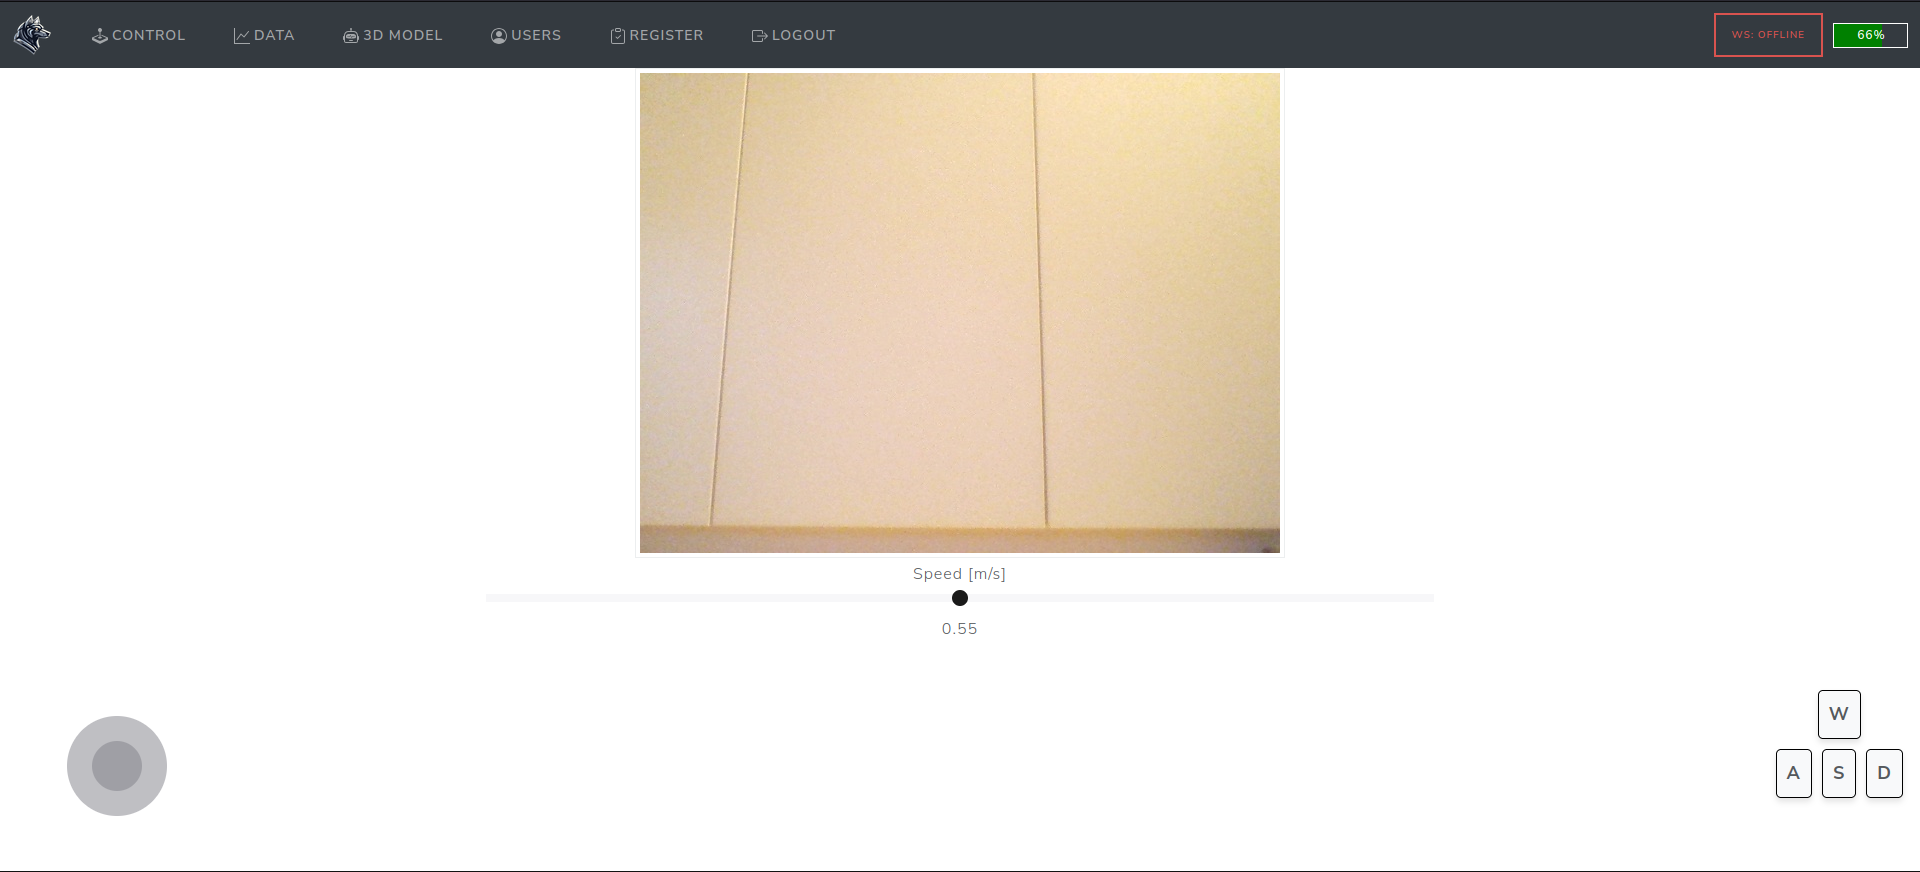
\includegraphics[width=0.98\columnwidth]{images/control_panel.png}}
    \caption{Control panel of the Web App with a navigation bar on top, camera stream in the center, control elements left and right and a speed slider to adjust the robot speed.}
    \label{fig:controlpanel}
\end{figure}
\subsection{Data panel}
The data panel in Fig. \ref{fig:overviewplots} shows critical live robot data such as the left and right motor temperatures as gauges. 
Furthermore, the temperatures and the battery SoC are shown in diagrams with time progression. 
The data for the visualization is provided by an SQLite database, which in turn reads the data from the respective ROS topics of the Husky. 
It is possible to select and visualize individual days in the diagrams and snapshots can be taken if required.

\begin{figure}[htbp]
    \centerline{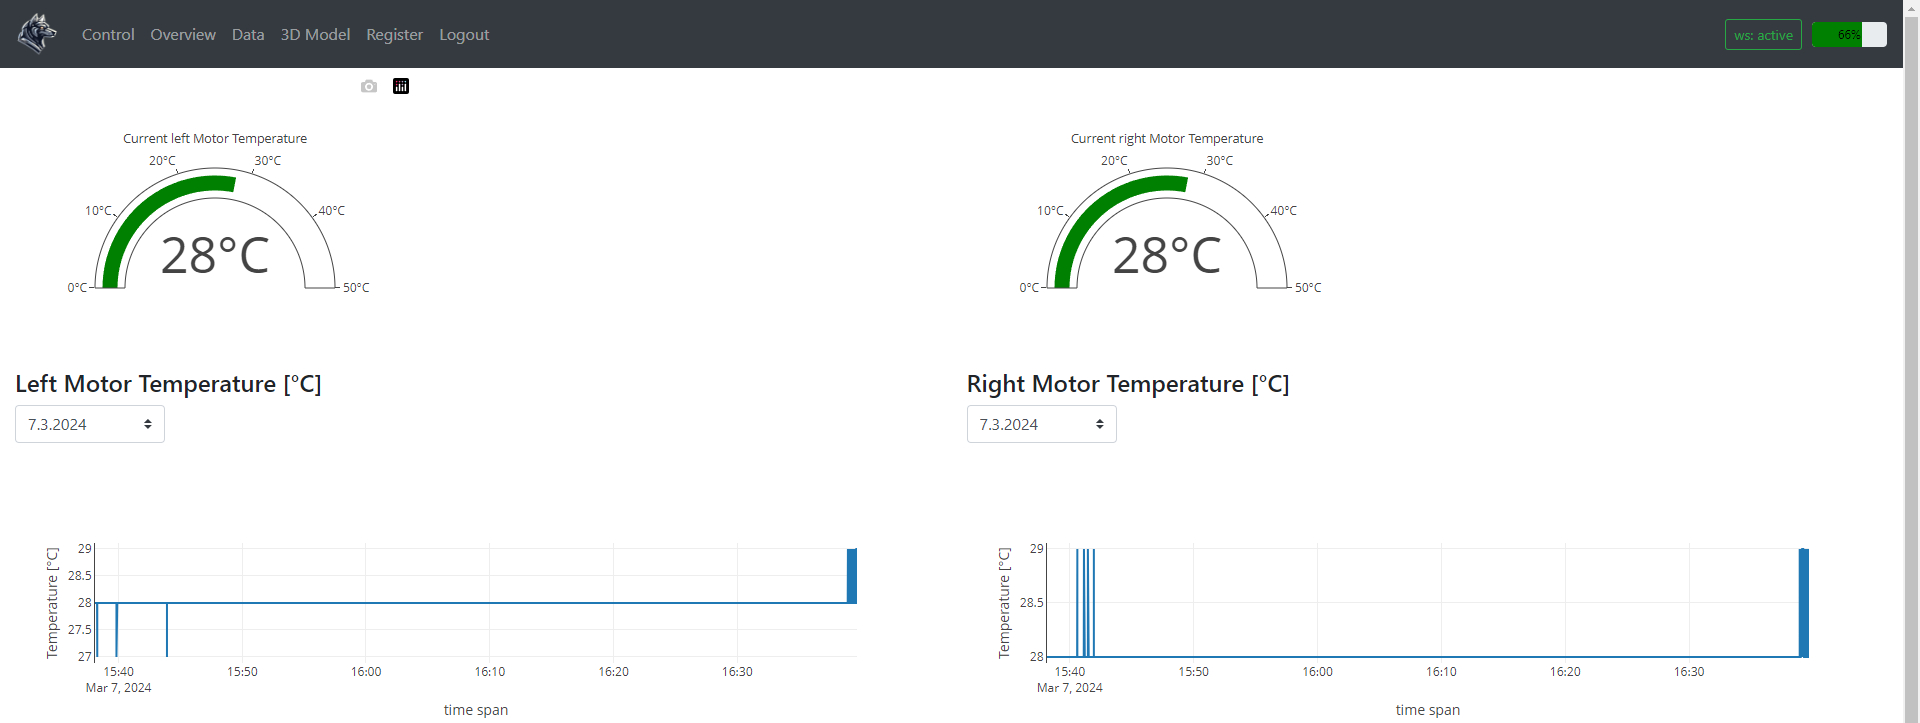
\includegraphics[width=8.9cm]{images/overviewplots.png}}
    \caption{Data panel with left and right motor temperatures which are ae presented live as gauges and historic data is presented via the SQLite database.}
    \label{fig:overviewplots}
\end{figure}

\subsection{Additional features and considerations}
Additional features of the framework include: 
\begin{itemize}
\item User login system for security purposes
\item Visualization of the Husky 3D model 
\item Database connection with a specially developed OPC-UA server, to store other robot data apart from the Husky
\end{itemize}
Bootstrap, a frontend framework, was leveraged to facillitate responsive web design \cite{bootstrap}. 
This allows control elements and data visualizations to be optimally displayed on mobile or desktop devices of the robot operator and ensures that the robot operator retains an overview and control of the robot.








\section{RELATED WORK}
% Geometric navigation approaches that are for example LiDAR based, are especially limited outdoors \cite{wayfast}.
% Self-supervised navigation systems such as BADGR \cite{BADGR}, WayFAST \cite{wayfast} or the successor model WayFASTER \cite{wayfaster}, are therefore used to estimate the traversability with regard to bumps and navigable objects such as tall grass.
% Even though they excel in a static environment, they are constrained in a dynamic and busy environment where people or other objects such as cars are moving.
% For that reason 
- Shared Autonomy
- Presentation of BADGR and WayFASTER
- Web based UI Apps?



\section{Methodology and Concept}
We propose a shared autonomy approach of the guidance of a robot such as the Husky UGV from Clearpath. 
The idea is to let the robot take over initial control through a self-supervised navigation system such as WayFASTER.
The kino-dynamic model of a skid-steered Robot, such as the Husky, is given below: \cite{wayfaster}
% by \eqref{eq:kino-model} \cite{wayfaster}.

\vspace{-0.1in}

% \begin{equation}
%     x_{k+1}
%     =
%     \begin{bmatrix}
%         p_{x_k} \\
%         p_{y_k} \\
%         \theta_k
%     \end{bmatrix}
%     +
%     \begin{bmatrix}
%         \mu \cdot cos(\theta_k) & 0 \\
%         \mu \cdot sin(\theta_k) & 0  \\
%         0 & \nu
%     \end{bmatrix}
%     \begin{bmatrix}
%         v_k \\
%         \omega_k
%     \end{bmatrix}
%     \cdot \Delta t
%     \label{eq:kino-model}
% \end{equation}

\begin{equation*}
    \resizebox{0.95\hsize}{!}{%
        % $\begin{bmatrix}
        %     p_{x_{k+1}} \\
        %     p_{y_{k+1}} \\
        %     \theta_{k+1}
        % \end{bmatrix}
        $x_{k+1}
        =
        \begin{bmatrix}
            p_{x_k} \\
            p_{y_k} \\
            \theta_k
        \end{bmatrix}
        +
        \begin{bmatrix}
            \mu(p_{x_k}, p_{y_k}) \cdot cos(\theta_k) & 0 \\
            \mu(p_{x_k}, p_{y_k}) \cdot sin(\theta_k) & 0  \\ 
            0 & \nu(p_{x_k}, p_{y_k})
        \end{bmatrix}
        \begin{bmatrix}
            v_k \\
            \omega_k
        \end{bmatrix}$
    }
    \label{eq:kino-model}
\end{equation*}

where $x_k$ is the state vector, $p_x$ and $p_y$ are the coordinates and $\theta_k$ is the orientation (heading angle) of the robot. 
The $cos(\theta_k)$ and $sin(\theta_k)$ functions describe the movement in x- and y-Axis depending on the orientation.
$\mu(p_x,p_y)$ and $\nu(p_x,p_y)$ are outputs (traversability coefficients) of the WayFASTER model TravNet and have a value between 1 and 0 respectively.
They indicate how well the robot can move across the terrain and are associated with the control inputs $v_k$ and $\omega_k$, which are the linear and angular velocities. 
In ROS terms are these are what a Twist Message contains.

We plan to integrate the transversability coefficients into our web framework. Since these coefficients have a value of 1 for good transversability and 0 for poor transversability, a threshold can be specified. 
A value of 0 (for both coefficients) would mean that the robot stops. To ensure a more seamless transition from autonomous control to human control, falling below the defined threshold will result in a warning in the web app.
This is intended to indicate the human operator to take control within the app. The app is programmed in such a way that human input always has top priority. Specifically, this can be achieved with Husky by sending control commands (geometry\_msgs/Twist\_Message) in different topics with different priorities [source]. 

%Vom Wayfaster Paper: "The estimator uses the discrete system model shown in \eqref{eq:kino-model} and synchronously runs with the GNSS module on the robot at a sampling time $\Delta t$. We solve the following finite horizon optimization formulation to obtain the system states and unknown parameters $\mu$ and $\nu$."



   \begin{figure}[thpb]
      \centering
      \framebox{\parbox{3in}{We suggest that you use a text box to insert a graphic (which is ideally a 300 dpi TIFF or EPS file, with all fonts embedded) because, in an document, this method is somewhat more stable than directly inserting a picture.
}}
      %\includegraphics[scale=1.0]{figurefile}
      \caption{Inductance of oscillation winding on amorphous
       magnetic core versus DC bias magnetic field}
      \label{figurelabel}
   \end{figure}
   


\section{Transversability-Based Shared Control}
\begin{figure}[htbp]
	\centerline{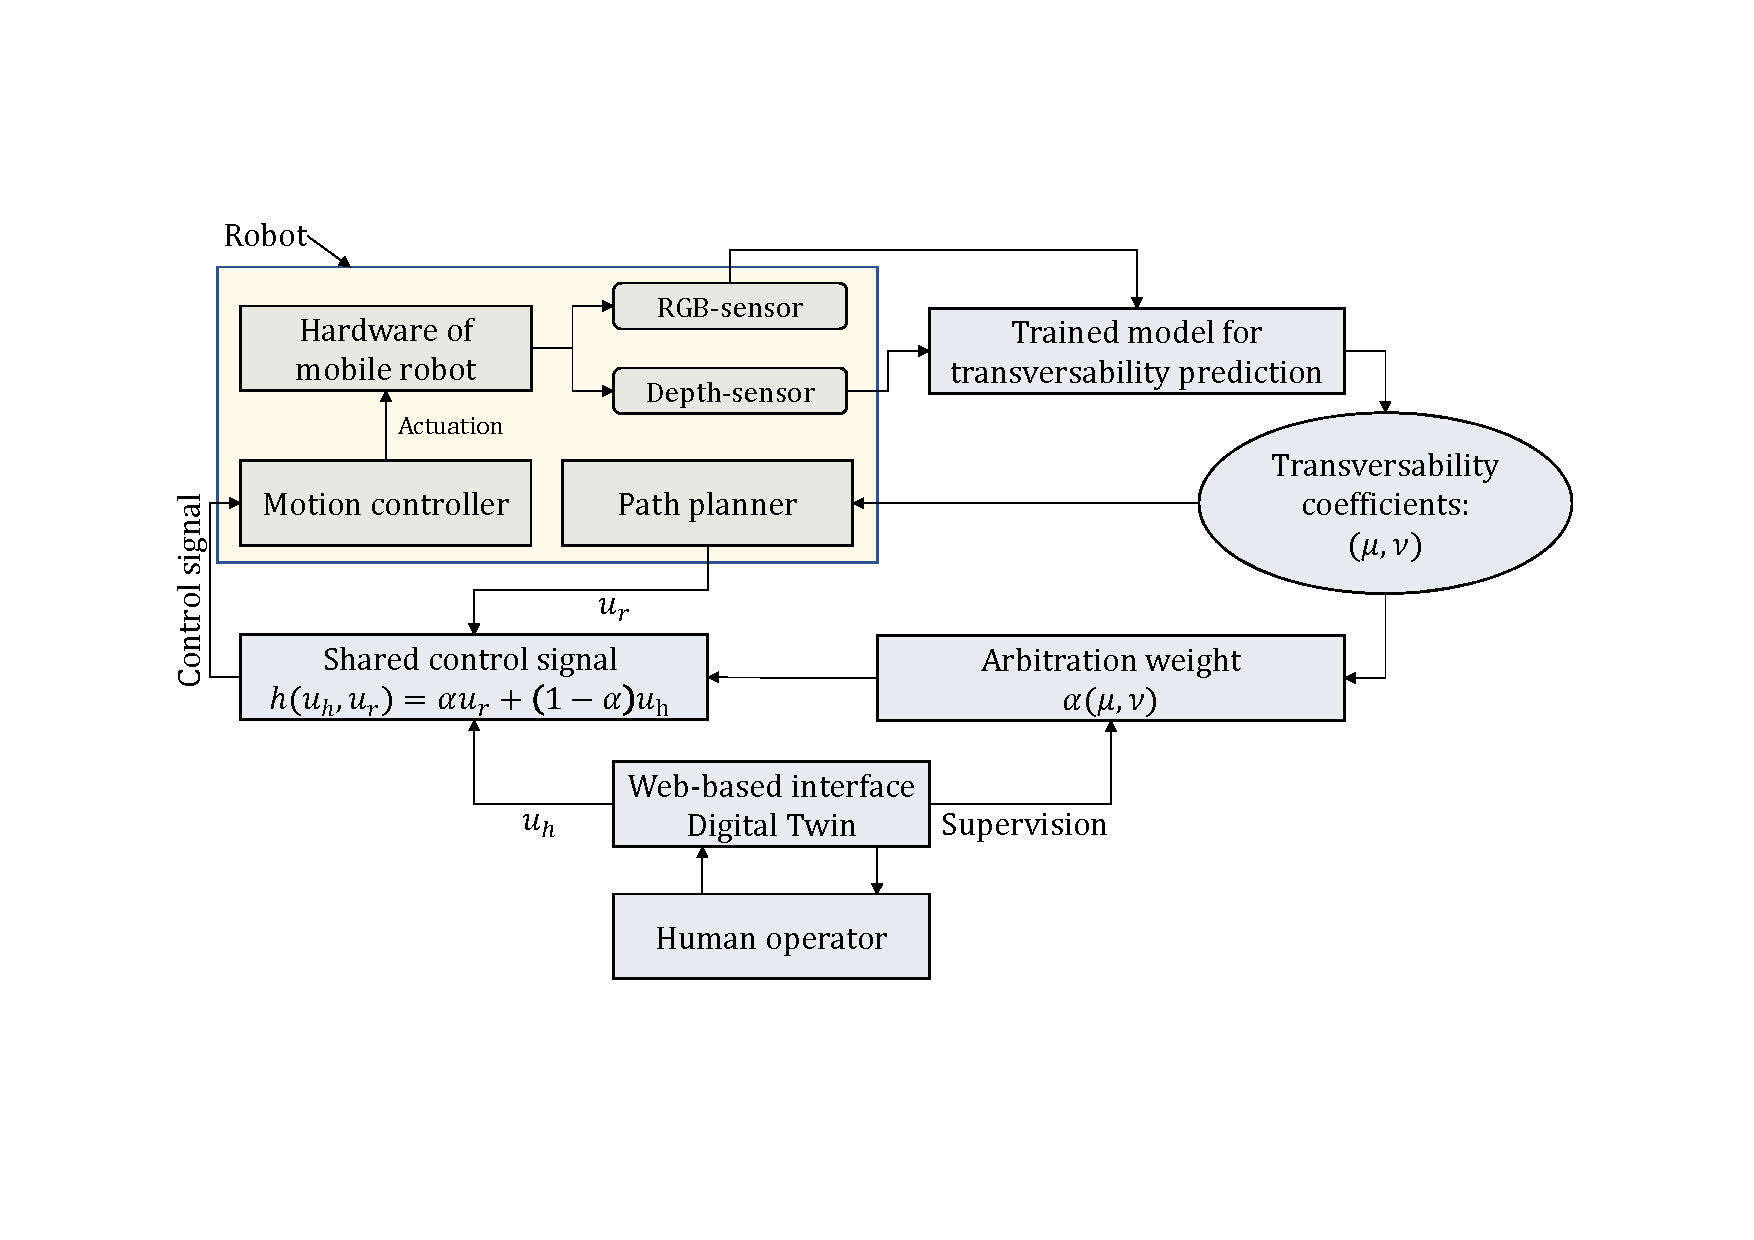
\includegraphics[width=8.9cm]{images/transversability.pdf}}
	\caption{Shared Control}
	\label{fig:sharedcontrol}
\end{figure}
\section{CONCLUSIONS}


\addtolength{\textheight}{-12cm}   % This command serves to balance the column lengths
                                  % on the last page of the document manually. It shortens
                                  % the textheight of the last page by a suitable amount.
                                  % This command does not take effect until the next page
                                  % so it should come on the page before the last. Make
                                  % sure that you do not shorten the textheight too much.

%%%%%%%%%%%%%%%%%%%%%%%%%%%%%%%%%%%%%%%%%%%%%%%%%%%%%%%%%%%%%%%%%%%%%%%%%%%%%%%%



%%%%%%%%%%%%%%%%%%%%%%%%%%%%%%%%%%%%%%%%%%%%%%%%%%%%%%%%%%%%%%%%%%%%%%%%%%%%%%%%



%%%%%%%%%%%%%%%%%%%%%%%%%%%%%%%%%%%%%%%%%%%%%%%%%%%%%%%%%%%%%%%%%%%%%%%%%%%%%%%%




\begin{thebibliography}{99}

\bibitem{wayfast} M. V. Gasparino et al., "WayFAST: Navigation With Predictive Traversability in the Field," in IEEE Robotics and Automation Letters, vol. 7, no. 4, pp. 10651-10658, Oct. 2022, doi: 10.1109/LRA.2022.3193464.
\bibitem{BADGR} G. Kahn, P. Abbeel and S. Levine, "BADGR: An Autonomous Self-Supervised Learning-Based Navigation System," in IEEE Robotics and Automation Letters, vol. 6, no. 2, pp. 1312-1319, April 2021, doi: 10.1109/LRA.2021.3057023.
\bibitem{wayfaster} M. V. Gasparino et al., "WayFASTER: a Self-Supervised Traversability Prediction for Increased Navigation Awareness," Feb. 2024 arXiv preprint arXiv:2402.00683.
\bibitem{phri} M. Selvaggio, M. Cognetti, S. Nikolaidis, S. Ivaldi and B. Siciliano, "Autonomy in Physical Human-Robot Interaction: A Brief Survey," in IEEE Robotics and Automation Letters, vol. 6, no. 4, pp. 7989-7996, Oct. 2021, doi: 10.1109/LRA.2021.3100603.
\bibitem{husky}https://clearpathrobotics.com/husky-unmanned-ground-vehicle-robot/
\bibitem{bootstrap}"Introduction," Bootstrap, https://getbootstrap.com/docs/5.3/getting-started/introduction/ (accessed Aug. 9, 2024).
\bibitem{rosbridgeSuite}"rosbridge\_suite," rosbridge suite - ROS Wiki, http://wiki.ros.org/rosbridge\_suite (accessed March 14, 2024).
% \bibitem{energy} https://ieeexplore.ieee.org/stamp/stamp.jsp?tp=&arnumber=9808373
% \bibitem{seamless} https://ieeexplore.ieee.org/stamp/stamp.jsp?tp=&arnumber=9372861






\end{thebibliography}




\end{document}
